\documentclass{beamer}

%% \documentclass[handout]{beamer}
%% % use this with the [handout] option to create handouts for the audience
%% \usepackage{pgfpages}
%% \pgfpagesuselayout{2 on 1}[a4paper,border shrink=5mm]

\mode<presentation>
{
  \usetheme{Diku}
% set this to your preferences:
  \setbeamercovered{invisible}
%  \setbeamercovered{transparent}
}

\usepackage{graphicx}
\usepackage{epic}

\usepackage{amsmath}
\usepackage{amssymb}
\usepackage{amsthm}

\newcommand{\basetop}[1]{\vtop{\vskip-1ex\hbox{#1}}}
\newcommand{\source}[1]{\let\thefootnote\relax\footnotetext{\scriptsize\textcolor{kugray1}{Source: #1}}}

% for coloured code citation in text:
\usepackage{fancyvrb}

%%%%%%%%%%%%%%%%%%%%%%%%%%%%%%%%%
%%%%%    code sections   %%%%%%%%
%%%%%%%%%%%%%%%%%%%%%%%%%%%%%%%%%

% code highlighting commands in own block
\DefineVerbatimEnvironment{code}{Verbatim}{fontsize=\scriptsize}
\DefineVerbatimEnvironment{icode}{Verbatim}{fontsize=\scriptsize}

% Fancy code with color commands:
\DefineVerbatimEnvironment{colorcode}%
        {Verbatim}{fontsize=\scriptsize,commandchars=\\\{\}}

%%%%%%%%%%%%%%%%%%%%%%%%%%%%%%%%%%
%%%%%    some coloring    %%%%%%%%

\definecolor{Red}{RGB}{220,50,10}
\definecolor{Blue}{RGB}{0,51,102}
\definecolor{Yellow}{RGB}{102,51,0}
\definecolor{Orange}{RGB}{178,36,36}
\definecolor{Grey}{RGB}{180,180,180}
\definecolor{Green}{RGB}{20,120,20}
\definecolor{Purple}{RGB}{160,50,100}
\newcommand{\red}[1]{\textcolor{Red}{{#1}}}
\newcommand{\blue}[1]{\textcolor{Blue}{{#1}}}
\newcommand{\yellow}[1]{\textcolor{Yellow}{{#1}}}
\newcommand{\orange}[1]{\textcolor{Orange}{{#1}}}
\newcommand{\grey}[1]{\textcolor{Grey}{{#1}}}
\newcommand{\green}[1]{\textcolor{Green}{{#1}}}
\newcommand{\purple}[1]{\textcolor{Purple}{{#1}}}




% use "DIKU green" from our color theme for \emph
\renewcommand{\emph}[1]{\textcolor{structure}{#1}}
% use some not-too-bright red for an \emp command
\definecolor{DikuRed}{RGB}{130,50,32}
\newcommand{\emp}[1]{\textcolor{DikuRed}{ #1}}
\definecolor{CosGreen}{RGB}{10,100,70}
\newcommand{\emphh}[1]{\textcolor{CosGreen}{ #1}}
\definecolor{CosBlue}{RGB}{55,111,122}
\newcommand{\emphb}[1]{\textcolor{CosBlue}{ #1}}
\definecolor{CosRed}{RGB}{253,1,1}
\newcommand{\empr}[1]{\textcolor{CosRed}{ #1}}

\newcommand{\mymath}[1]{$ #1 $}
\newcommand{\myindx}[1]{_{#1}}
\newcommand{\myindu}[1]{^{#1}}

\newcommand{\Fasto}{\textsc{Fasto}\xspace}


%%%%%%%%%%%%%%%%%%%%

\title[Assignments]{First and Second Assignments Discussion}

\author[C.~Oancea]{Cosmin E. Oancea {\tt cosmin.oancea@diku.dk}}

\institute{Department of Computer Science (DIKU)\\University of Copenhagen}


\date[Sept 2014]{September 2014 PMPH Lecture Notes}


\begin{document}

\titleslide


\section{Assignment 1}

\begin{frame}[fragile]
	\tableofcontents[currentsection]
\end{frame}


\begin{frame}[fragile,t]
\frametitle{Common Missunderstandings}

\begin{itemize}
    \item ``Task 4 from Assignment 1 is not well specified!''\\\pause
        \begin{itemize}
            \item It is intentionally underspecified because of the
            \item Context: Programming Models to Exploit Hardware Parallelism. 
            \item expecting \emp{best Work and Depth asymptotic AND flat parallelism.}  
        \end  {itemize}\medskip
    \item I apologize to the students whose code I am going to show,
%    \item I only show it for didactic purposes, so that we all learn,
    \item I actually picked the ones that were close(r) to a correct solution,
    \item and I am sure that most of them were thought as a partial implementation...
%\medskip

%    \item \alert{Do I have your permission to show some of them in didactic purposes?}

\end  {itemize}
\end{frame}

\begin{frame}[fragile,t]
\frametitle{But ... my Haskell Program Works (?)}

Haskell used just as a vehicle to reason about ``parallelism''
in terms of bulk, parallel primitive operators: 
map, reduce, scan, permute, write.\pause\medskip

\begin{colorcode}[fontsize=\scriptsize]
 flatSparseMatVctMult flags mat x = 
    let vec_os  = \emph{map (\mymath{\backslash}n -> n-1) \$ scanInc (+) 0 flags}
        tmp_mat = \emph{segmScanInc (+) 0 flags \$ map (\mymath{\backslash}(col,val) -> x!!col * val) mat}
    in \alert{extract_result vec_os tmp_mat}
extract_result :: [Int] -> [a] -> [a]
extract_result flags mat = let 
    extract_result_inner [] [] _ = []
    extract_result_inner [x] [z] tmpres = tmpres++[z]
    \alert{extract_result_inner} (x:y:xs) (z:zs) tmpres = 
        if x /= y
        then \alert{extract_result_inner} (y:xs) zs (tmpres++[z])
        else \alert{extract_result_inner} (y:xs) zs tmpres
    extract_result_inner _ _ _ = []
  in extract_result_inner flags mat []
\end{colorcode}

\end{frame}


\begin{frame}[fragile,t]
\frametitle{But ... my Haskell Program Works (?)}

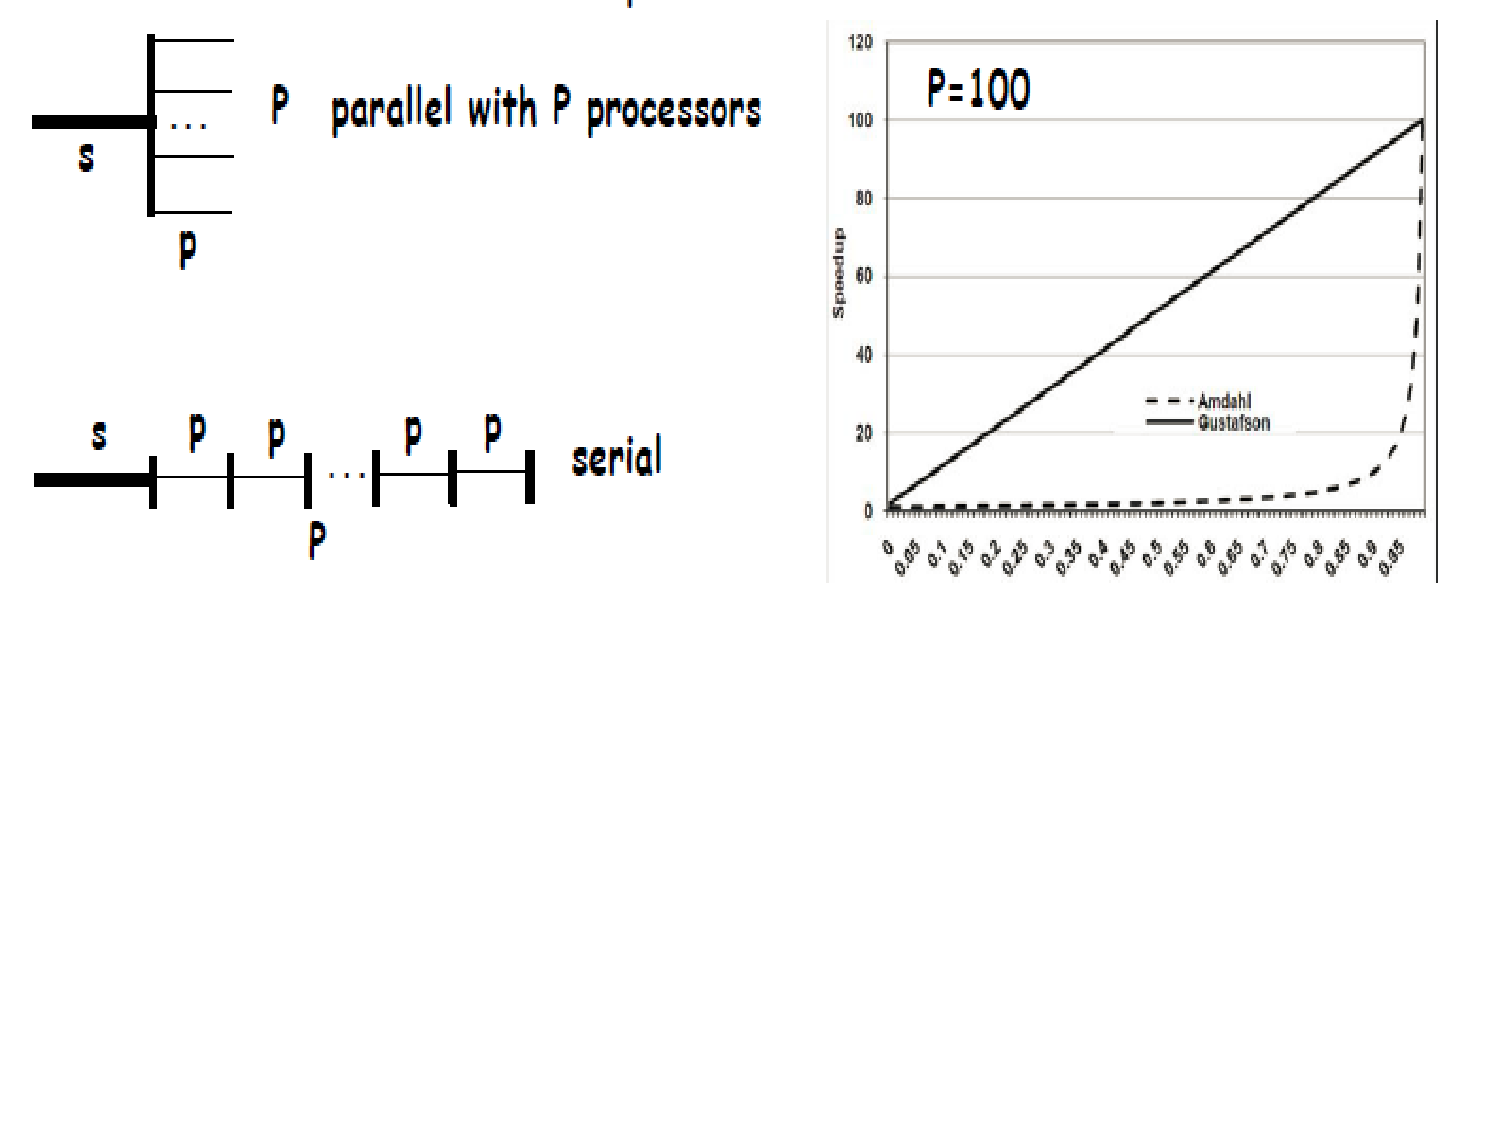
\includegraphics[width=59ex]{Ch1Figs/AmdhalGustaff}
\vspace{-15ex}

\alert{Remember: Amdhal's low is unforgiving}: if  
{\tt extract\_results} takes a third of sequential 
exec time, what is the maximal speedup?
\medskip

You might get partial marks, but little performance gain!

\end{frame}

\begin{frame}[fragile,t]
\frametitle{But ... I Like My Foldl/Scanl (?)}

\begin{colorcode}[fontsize=\scriptsize]
nestSparseMatVctMult mat x = 
    map (\mymath{\backslash}row -> let (_,yi) = reduce (\mymath{\backslash}(_,acc) (i,v2) ->
                                           \alert{(0, acc + v2*(x !! i))}
                                     ) (0,0.0) row
             in yi
        ) mat
\end{colorcode}
\pause

Semantically a {\tt foldl :: (a -> b -> a) -> a -> [b] -> a}

\medskip
Monoids $\Rightarrow$ Homomorphism $\Rightarrow$ ...
\alert{Neutral elem \& associative op}.\medskip

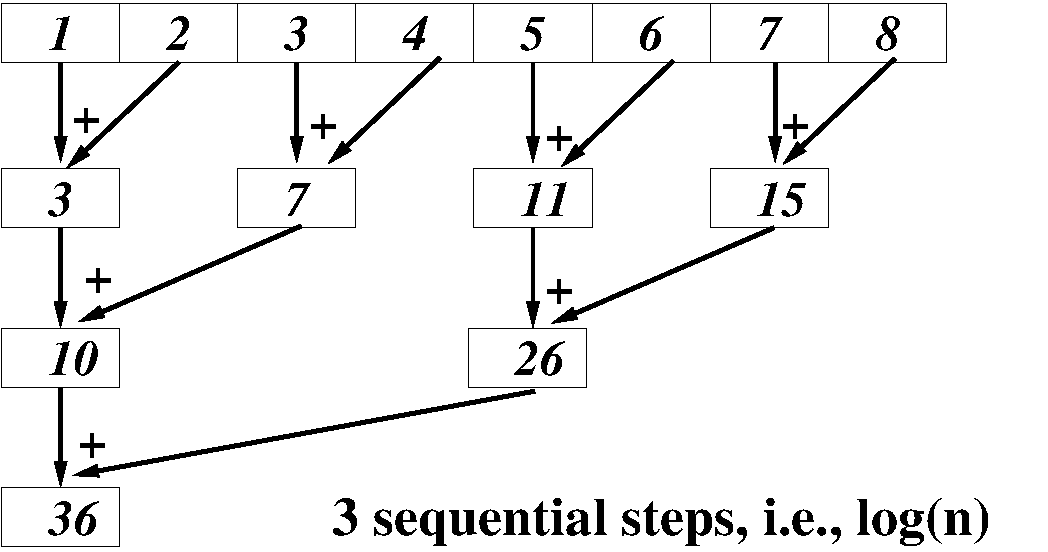
\includegraphics[height=22ex]{Figures/ReduceEg.pdf} 

Remember: CISC vs RISC (simple is good)!

\end{frame}


\begin{frame}[fragile,t]
\frametitle{But ... My Scan Operator Is Associative (?)}

\begin{colorcode}[fontsize=\scriptsize]
segmScanInc (\mymath{\backslash}(c1,(on1,en1),(o1,e1)) (c2,(on2,en2),(o2,e2)) -> 
                if c1 then (c2,(on1+on2,en1+en2),(o1\alert{++}o2,e1\alert{++}e2)) 
                else (c1,(on1+on2,en1+en2),(o1\alert{++}o2,e1\alert{++}e2))) 
            (True,(0,0),([],[])) sizes zipper
\end{colorcode}
\medskip

Merge operator using concatenate is in most cases inefficient!

\end{frame}


\section{Scan and Segmented Scan on GPU}

\subsection{Scan}

\begin{frame}[fragile]
	\tableofcontents[currentsubsection]
\end{frame}


\begin{frame}[fragile,t]
\frametitle{{\tiny Scan Implementation: Slide From CMU 15-418 Parallel Computer Architecture and Programming}}

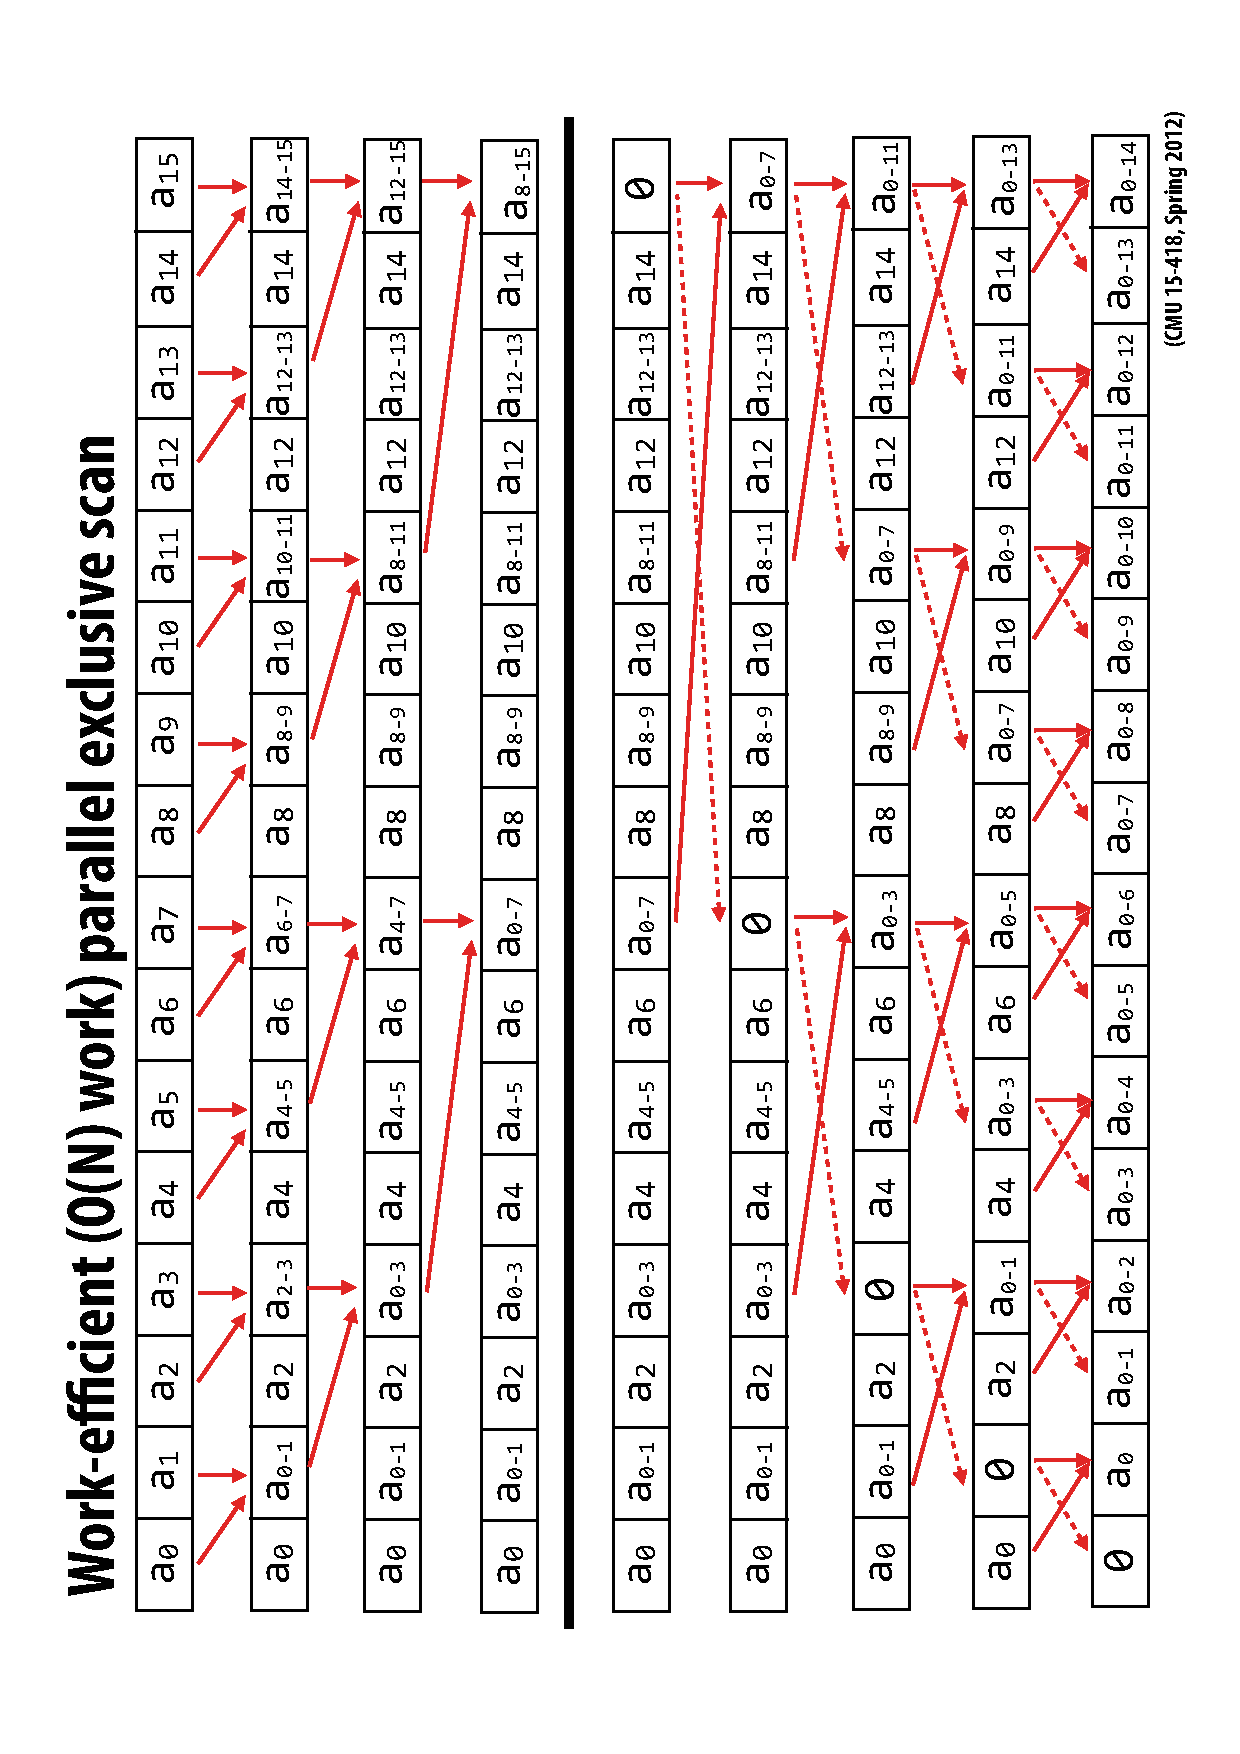
\includegraphics[width=55ex]{Figures/ExcScanNew}

\end{frame}

\begin{frame}[fragile,t]
\frametitle{{\tiny GPU Warp Scan Implem: Slide From CMU 15-418 Parallel Computer Architecture and Programming}}

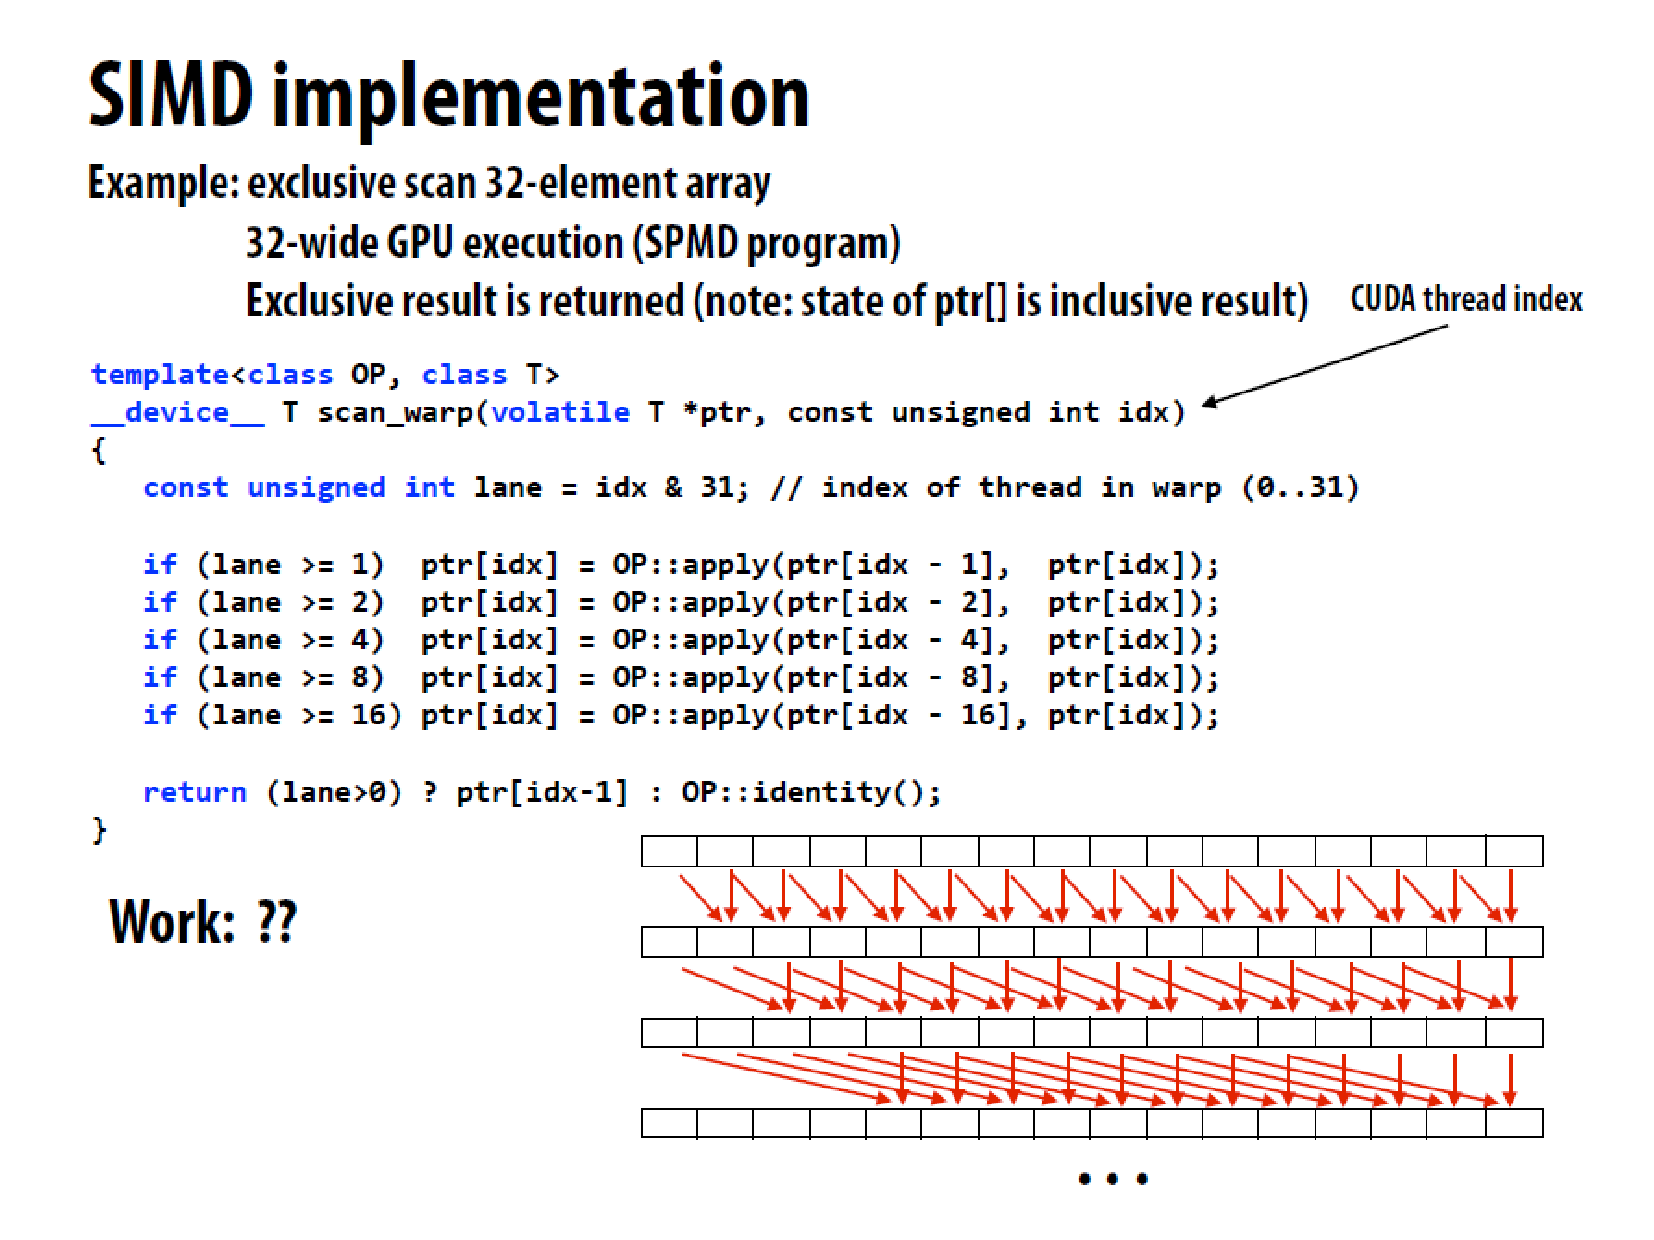
\includegraphics[width=55ex]{Figures/ExcScanGPU}

\end{frame}


\begin{frame}[fragile,t]
\frametitle{GPU Scan Implementation}
\begin{itemize}
    \item[-] \alert{work inefficient} O(N lg N)
    \item[+] but the work efficient algorithm 
                would result in low GPU utilization, 
                i.e.,  would require $>$ $2\times$ number of instructions.
    \item[+] better locality of reference.
    \item[+] no synchronization inside a {\sc warp}, due to {\sc simd} execution.
\end  {itemize}
\end{frame}

\begin{frame}[fragile,t]
\frametitle{{\tiny GPU Block Scan Implem: Slide From CMU 15-418 Parallel Computer Architecture and Programming}}

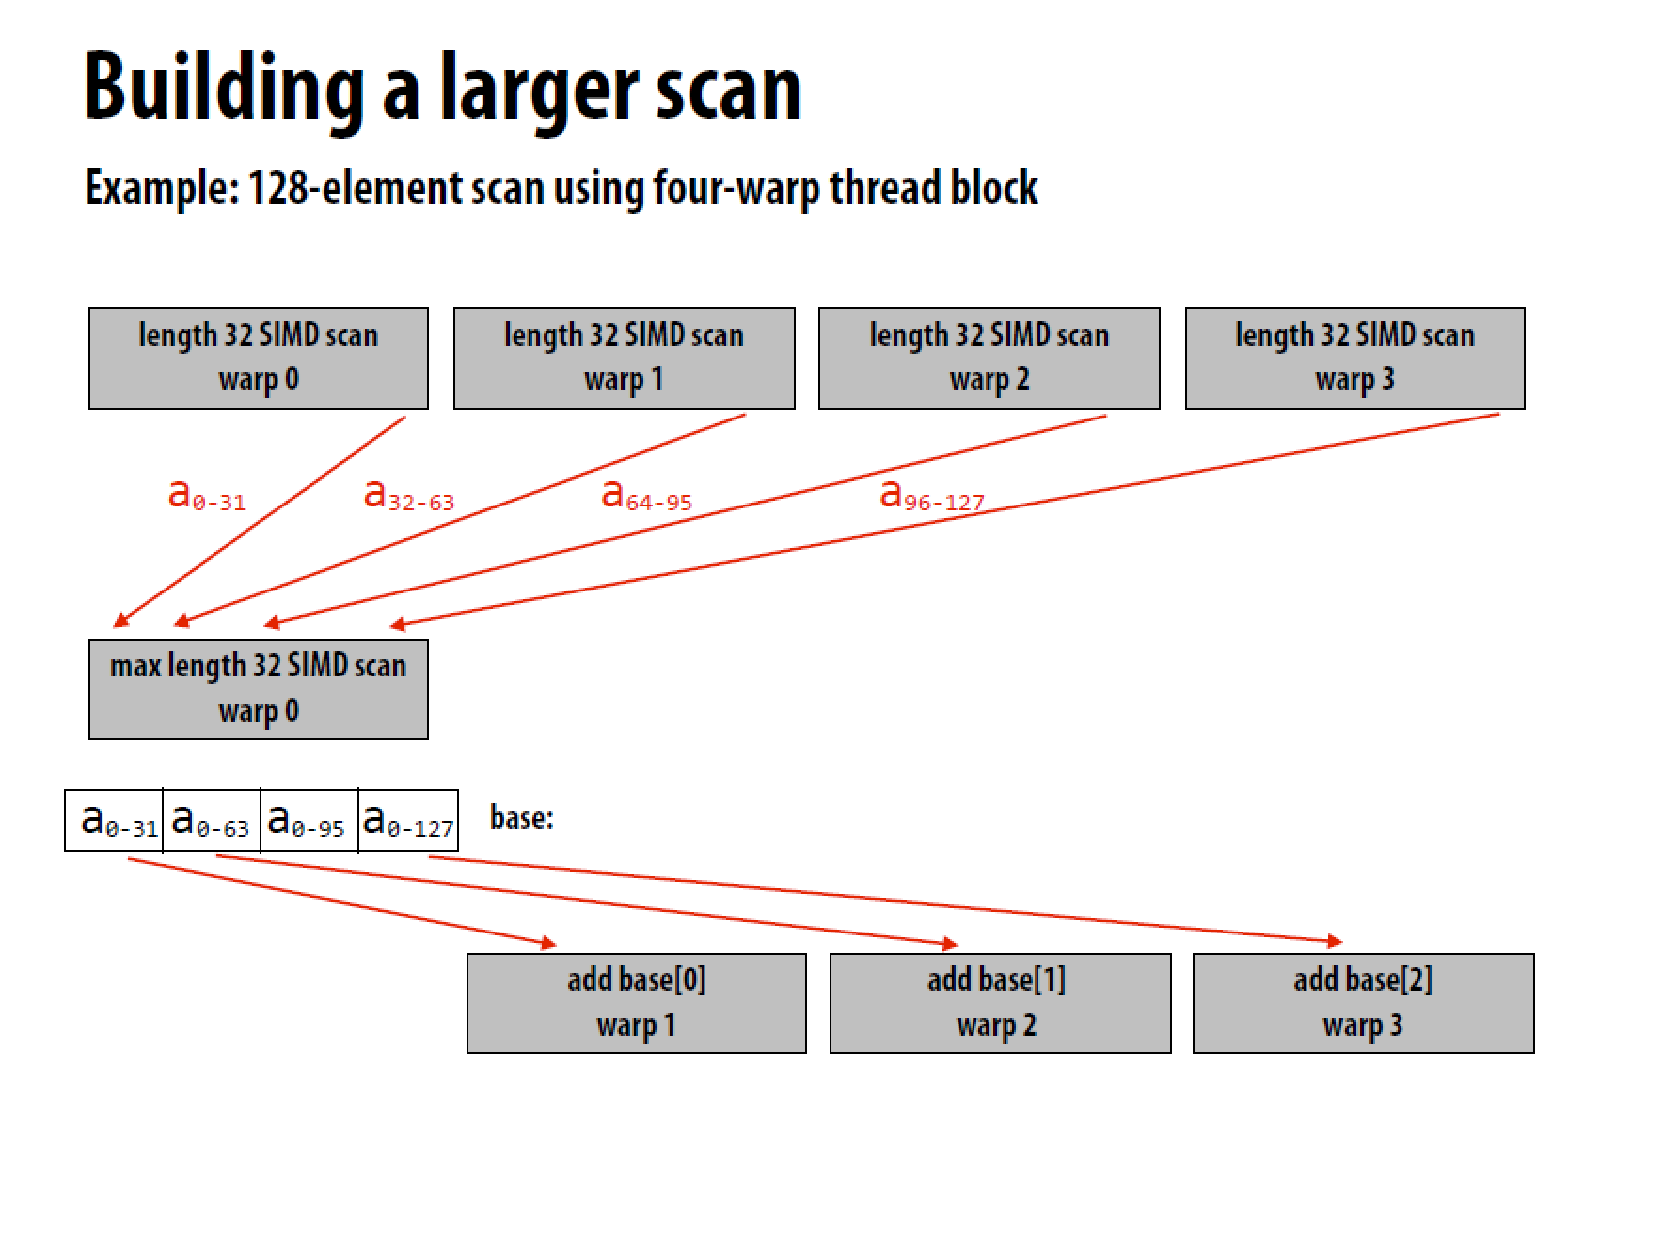
\includegraphics[width=55ex]{Figures/BlockScan}

\end{frame}

\begin{frame}[fragile,t]
\frametitle{GPU Block-Level Scan Implementation}

A warp is formed by 32 threads and a block has at most $32^2=1024$ threads $\Rightarrow$we need only two steps to perform the scan at block level!\medskip

\begin{colorcode}[fontsize=\scriptsize]
template<class OP, class T>
__device__ T 
scanExcBlock(volatile T* ptr, const unsigned int idx) \{
    const unsigned int lane   = idx &  31;
    const unsigned int warpid = idx >> 5;

    T val = scanExcWarp<OP,T>(ptr,idx);
    __syncthreads(); \emph{//scan all warps in parallel}

    if (lane == 31) ptr[warpid] = ptr[idx]; 
    __syncthreads(); \emph{//record the last partial result of each warp}

    if (warpid == 0) scanExcWarp<OP,T>(ptr, idx);
    __syncthreads(); \emph{//First warp performs scan on the partial result}

    if (warpid > 0) \emph{//each thread accumulates the partial results}
        val = OP::apply(ptr[warpid-1], val);

    return val;
\}
\end{colorcode}

\end{frame}


\begin{frame}[fragile,t]
\frametitle{GPU Application-Level Scan Implementation}

If array size $<$ one GPU block, then enough!\\
Otherwise apply recursively!\medskip


\begin{colorcode}[fontsize=\tiny]
template<class OP, class T>
void scanIncAdd( int block_size, int d_size, T* d_in, T* d_out ) \{
    // ...
    \emph{scanIncKernel<OP,T><<< num_blocks, block_size, sh_mem_size >>>(d_in, d_out, d_size);}
    cudaThreadSynchronize();
    
    \alert{if (block_size >= d_size) { return; }}  // Recursive Case follows:

    //   1. allocate new device input & output array of size num_blocks
    T *d_rec_in, *d_rec_out;
    cudaMalloc((void**)&d_rec_in , num_blocks*sizeof(T));
    cudaMalloc((void**)&d_rec_out, num_blocks*sizeof(T)); // ...
    
    //   2. copy in the end-of-block results of the previous scan 
    copyEndOfBlockKernel<T><<< num_blocks_rec, block_size >>>(d_out, d_rec_in, num_blocks);
    //   3. scan recursively the last elements of each CUDA block
    \alert{scanIncAdd<OP,T>( block_size, num_blocks, d_rec_in, d_rec_out );}

    //   4. distribute each of the recursively scanned elements 
    distributeEndBlock<T><<< num_blocks, block_size >>>(d_rec_out, d_out, d_size);
\}
\end{colorcode}

\end{frame}

\begin{frame}[fragile,t]
\frametitle{How to Call It?}

\begin{colorcode}[fontsize=\scriptsize]

template<class T>
class Add \{
  public:
    static __device__ T identity()        \{ return (T)0;    \}
    static __device__ T apply(T t1, T t2) \{ return t1 + t2; \}
\};

int main(...) \{ 
    ...
    \emph{sgmScanIncAdd< Add<float>,float >}
        ( 512, num_threads, d_in, flags_d, d_out );\
    ...
\}
\end{colorcode}
\end{frame}

\subsection{Segmented Scan}

\begin{frame}[fragile]
	\tableofcontents[currentsubsection]
\end{frame}


\begin{frame}[fragile,t]
\frametitle{GPU Warp-Level Segmented Scan}

{\tt(f$_x$,x) $\oplus$ (f$_y$,y) = (f$_x$.|.f$_y$, if f$_y$ then y else x $\oplus$ y)}
\medskip

S. Sengupta, M. Harris, Y. Zhang, and J. D. Owens. {\em Scan primitives for GPU computing.} In Graphics Hardware 2007, pages 97-106, 2007.\medskip

\begin{colorcode}[fontsize=\scriptsize]
template<class OP, class T, class F> __device__ T 
sgmScanIncWarp(volatile T* ptr, volatile F* flg, const unsigned int idx) \{
  const unsigned int lane = idx & 31;
  if (lane >= 1)  \{
    ptr[idx] = (flg[idx] != 0) ? ptr[idx] : OP::apply(ptr[idx-1],  ptr[idx]);
    flg[idx] = flg[idx-1] | flg[idx];
  \}
  if (lane >= 2)  \{
    ptr[idx] = (flg[idx] != 0) ? ptr[idx] : OP::apply(ptr[idx-2],  ptr[idx]);
    flg[idx] = flg[idx-2] | flg[idx];
  \}
  // ... same with -4, and -8 ...
  if (lane >= 16)  \{
    ptr[idx] = (flg[idx] != 0) ? ptr[idx] : OP::apply(ptr[idx-16],  ptr[idx]);
    flg[idx] = flg[idx-16] | flg[idx];
  \}
  return ptr[idx];
\}
\end{colorcode}

\end{frame}


\begin{frame}[fragile,t]
\frametitle{GPU Warp-Level Segmented Scan}

{\tt(f$_x$,x) $\oplus$ (f$_y$,y) = (f$_x$.|.f$_y$, if f$_y$ then y else x $\oplus$ y)}
\medskip

The ``or'' between flags answers the question: 
is there a segment boundary to the left?\medskip
%within the warp?

To implement at block level:
\begin{itemize}
    \item The result flag answers if there is a segment boundary in the 
            warp to the left of the current thread,\smallskip
    \item The flag for the partial scan would correspond to the
            result flag of the last element in the warp.\smallskip
    \item Evaluate the partial scan in the first warp (only). 
           This is enough because warp size is $32$ and block size
            is at most $32^2=1024$\smallskip
    \item Finally each thread accumulates the partial result 
            if and only if the warp is open and there is no
            segment boundary to the left.
\end  {itemize}
\end{frame}

\begin{frame}[fragile,t]
\frametitle{GPU Block-Level Segmented Scan Implementation}

\begin{colorcode}[fontsize=\tiny]
template<class OP, class T, class F> __device__ T 
sgmScanIncBlock(volatile T* ptr, volatile F* flg, const unsigned int idx) \{
    const unsigned int lane   = idx &  31, warpid = idx >> 5;
    const unsigned int warplst= (warpid<<5) + 31;

    // \emp{1a: record whether this warp begins with an ``open'' segment.}
    bool warp_is_open = (flg[(warpid << 5)] == 0); 
    __syncthreads();

    // \emp{1b: intra-warp segmented scan for each warp}
    T val = sgmScanIncWarp<OP,T>(ptr,flg,idx);

    // \emp{2a: the last value is the correct partial result}
    T warp_total = ptr[warplst];
    
    // \emp{2b: warp_flag is the OR-reduction of the flags in a warp}
    bool warp_flag = flg[warplst]!=0 || !warp_is_open;
    bool will_accum= warp_is_open && (flg[idx] == 0); 
    __syncthreads();

    // \emp{2c: the last thread in a warp writes partial results}
    if (lane == 31) \{ ptr[warpid] = warp_total; flg[warpid] = warp_flag; \}
    __syncthreads();

    if (warpid == 0) sgmScanIncWarp<OP,T>(ptr, flg, idx);
    __syncthreads();
    // \emp{4. accumulates if warp is open \&\& no segment boundary to its left}
    if (warpid > 0 && will_accum) val = OP::apply(ptr[warpid-1], val);
    return val;
\}
\end{colorcode}

\end{frame}

\begin{frame}[fragile,t]
\frametitle{GPU Application-Level Segmented Scan}

If array size $<$ one GPU block, then enough!\\
Otherwise apply recursively!\medskip


\begin{colorcode}[fontsize=\tiny]
template<class OP, class T, class OP_INT>
void sgmScanIncAdd( unsigned int  block_size, unsigned long d_size, 
                    T* d_in,  int* flags, T* d_out ) \{  
    .... // block-level scan
    \emph{sgmScanIncKernel <<< num_blocks, block_size, val_sh_size+flg_sh_size >>>}
                    \emph{(d_in, flags, d_out, f_rec_in, d_rec_in, d_size);}
    cudaThreadSynchronize(); 

    if (block_size >= d_size) { /*...*/ return; }  \emph{// recursion necessary?}

    //   1. allocate new device input & output array of size num_blocks
    T   *d_rec_out; int *f_inds;
    cudaMalloc((void**)&d_rec_out, num_blocks*sizeof(T   ));
    cudaMalloc((void**)&f_inds,    d_size    *sizeof(int ));

    //   2. recursive segmented scan on the last elements of each CUDA block
    \alert{sgmScanIncAdd<OP,T,OP_INT>( block_size, num_blocks, d_rec_in, f_rec_in, d_rec_out );}

    \emp{//   3. after scan inclusive at block level, f_inds will contain zeroes}
    \emp{//          only for the threads that are in the first segment of an open block!}
    \emp{scanIncKernel<OP_INT,int><<<num_blocks, block_size, flg_sh_size>>>(flags, f_inds, d_size);}

    //   4. finally, accumulate the recursive result of segmented scan
    //      to the elements from the first open segment of each block 
    sgmDistributeEndBlock<<< num_blocks, block_size >>>(d_rec_out, d_out, f_inds, d_size);

    //   5. clean up ...
\}
\end{colorcode}

\end{frame}


\section{Assignment 2}

\begin{frame}[fragile]
	\tableofcontents[currentsection]
\end{frame}


\begin{frame}[fragile,t]
\frametitle{Assignment 2}

\begin{itemize}
    \item[1] Implement {\bf quickly} exclusive scan and exclusive
                segmented scan\pause
             \begin{itemize}
                \item at this stage we only worry about asymptotic,
                        not targeting the best performance.
                \item since inclusive (segmented) scan is provided
                        how can you quickly derive an exclusive scan?
                      \emph{Hint: you can do it with a simple map!} 
             \end  {itemize}\medskip

    \item[2] Maximal Segment Sum Problem\pause
            \begin{itemize}
                \item there is a type int4 in CUDA (also float4 etc),\\
                        e.g., {\tt int4 v; v.x = 1; v.y = 2; v.z = 3; v.w = 4;}
                \item the last element of inclusive scan is the reduction,
                \item you just have to rewrite the operator that is passed to scan.
            \end  {itemize}\medskip

    \item[3] Implement one of the three problems.\pause
            \begin{itemize}
                \item now you understand why I have insisted on flat parallelism!
                \item you have the scans
                \item and need to write some maps 
                        (which are much simpler, like in the first assignment).
            \end  {itemize}
\end  {itemize}
\end{frame}

\begin{frame}[fragile,t]
\frametitle{One Can Implement Operators Other Than Add}

\begin{colorcode}[fontsize=\scriptsize]

template<class T>
class Add \{
  public:
    static __device__ T identity()        \{ return (T)0;    \}
    static __device__ T apply(T t1, T t2) \{ return t1 + t2; \}
\};

int main(...) \{ 
    ...
    \emph{sgmScanIncAdd< Add<float>,float >}
        ( 512, num_threads, d_in, flags_d, d_out );\
    ...
\}
\end{colorcode}
\end{frame}

\end{document}
